\documentclass{beamer}
\usetheme[pageofpages=of,% String used between the current page and the
                         % total page count.
          bullet=circle,% Use circles instead of squares for bullets.
          titleline=true,% Show a line below the frame title.
          alternativetitlepage=true,% Use the fancy title page.
	  titlepagelogo=logo-circl.pdf,% Logo for the first page.
%          watermark=watermark-polito,% Watermark used in every page.
%          watermarkheight=100px,% Height of the watermark.
%          watermarkheightmult=4,% The watermark image is 4 times bigger
                                % than watermarkheight.
          ]{Torino}

\usepackage[utf8x]{inputenc}
\usepackage{listings}
\usepackage{soul}
\usepackage{siunitx}
\usepackage{booktabs}
\usepackage{adjustbox}
%\lstset{ 
%  backgroundcolor=\color{white},   % choose the background color; you must add \usepackage{color} or \usepackage{xcolor}
%  basicstyle=\footnotesize,        % the size of the fonts that are used for the code
%  breakatwhitespace=false
%}

\usepackage{tikz}
\usetikzlibrary{shapes,snakes,automata,positioning,matrix,fit}


\usepackage[listings]{tcolorbox}
\usepackage{xcolor}
\usepackage{colortbl}
\definecolor{mygreen}{rgb}{0,0.6,0}
\definecolor{mygreen2}{rgb}{0,0.56,0.16}
\definecolor{myred}{rgb}{0.6,0.066,0.066}
\definecolor{redCIRCL}{RGB}{213,43,30}
\definecolor{mygray}{rgb}{0.5,0.5,0.5}
\definecolor{mymauve}{rgb}{0.58,0,0.82}
\definecolor{mygray}{gray}{0.9}
\definecolor{mywhite}{rgb}{1,1,1}
\definecolor{myblack}{rgb}{0,0,0}
\definecolor{mybeige}{HTML}{eeeeee}
%\usepackage{tcolorbox}
\usepackage[listings]{tcolorbox}
\tcbuselibrary{listings}

\lstdefinestyle{code}{ %
  backgroundcolor=\color{mybeige},   % choose the background color; you must add \usepackage{color} or \usepackage{xcolor}; should come as last argument
  basicstyle=\footnotesize\ttfamily,        % the size of the fonts that are used for the code
  breakatwhitespace=false,         % sets if automatic breaks should only happen at whitespace
  breaklines=true,                 % sets automatic line breaking
  captionpos=b,                    % sets the caption-position to bottom
  commentstyle=\color{mygreen},    % comment style
  deletekeywords={...},            % if you want to delete keywords from the given language
  escapeinside={\%*}{*)},          % if you want to add LaTeX within your code
  extendedchars=true,              % lets you use non-ASCII characters; for 8-bits encodings only, does not work with UTF-8
  frame=single,	                   % adds a frame around the code
  keepspaces=true,                 % keeps spaces in text, useful for keeping indentation of code (possibly needs columns=flexible)
  keywordstyle=\color{blue},       % keyword style
  language=Python,                 % the language of the code
  morekeywords={*,...},           % if you want to add more keywords to the set
  numbers=left,                    % where to put the line-numbers; possible values are (none, left, right)
  numbersep=5pt,                   % how far the line-numbers are from the code
  numberstyle=\tiny\color{myblack}, % the style that is used for the line-numbers
  rulecolor=\color{black},         % if not set, the frame-color may be changed on line-breaks within not-black text (e.g. comments (green here))
  showspaces=false,                % show spaces everywhere adding particular underscores; it overrides 'showstringspaces'
  showstringspaces=false,          % underline spaces within strings only
  showtabs=false,                  % show tabs within strings adding particular underscores
  stepnumber=1,                    % the step between two line-numbers. If it's 1, each line will be numbered
  stringstyle=\color{mymauve},     % string literal style
  tabsize=2,	                   % sets default tabsize to 2 spaces
  title=\lstname                   % show the filename of files included with \lstinputlisting; also try caption instead of title
}
\lstdefinestyle{bash}{ %
  backgroundcolor=\color{black!85},   % choose the background color; you must add \usepackage{color} or \usepackage{xcolor}; should come as last argument
  basicstyle=\footnotesize\color{mywhite},        % the size of the fonts that are used for the code
  breakatwhitespace=false,         % sets if automatic breaks should only happen at whitespace
  breaklines=true,                 % sets automatic line breaking
  captionpos=b,                    % sets the caption-position to bottom
  commentstyle=\color{mygreen},    % comment style
  deletekeywords={...},            % if you want to delete keywords from the given language
  escapeinside={\%*}{*)},          % if you want to add LaTeX within your code
  extendedchars=true,              % lets you use non-ASCII characters; for 8-bits encodings only, does not work with UTF-8
  frame=single	                   % adds a frame around the code
  keepspaces=true,                 % keeps spaces in text, useful for keeping indentation of code (possibly needs columns=flexible)
  keywordstyle=\color{white}\bfseries,       % keyword style
  language=bash,                 % the language of the code
  morekeywords={*,$,git, clone,... },           % if you want to add more keywords to the set
  numbers=left,                    % where to put the line-numbers; possible values are (none, left, right)
  numbersep=5pt,                   % how far the line-numbers are from the code
  numberstyle=\tiny\color{mywhite}, % the style that is used for the line-numbers
  rulecolor=\color{black},         % if not set, the frame-color may be changed on line-breaks within not-black text (e.g. comments (green here))
  showspaces=false,                % show spaces everywhere adding particular underscores; it overrides 'showstringspaces'
  showstringspaces=false,          % underline spaces within strings only
  showtabs=false,                  % show tabs within strings adding particular underscores
  stepnumber=1,                    % the step between two line-numbers. If it's 1, each line will be numbered
  stringstyle=\color{mymauve},     % string literal style
  tabsize=2,	                   % sets default tabsize to 2 spaces
  title=\lstname                   % show the filename of files included with \lstinputlisting; also try caption instead of title
}
\lstdefinestyle{default}{ %
  backgroundcolor=\color{white},   % choose the background color; you must add \usepackage{color} or \usepackage{xcolor}; should come as last argument
  basicstyle=\footnotesize\color{black},        % the size of the fonts that are used for the code
  breakatwhitespace=false,         % sets if automatic breaks should only happen at whitespace
  breaklines=true,                 % sets automatic line breaking
  captionpos=b,                    % sets the caption-position to bottom
  commentstyle=\color{mygreen},    % comment style
  deletekeywords={...},            % if you want to delete keywords from the given language
  escapeinside={\%*}{*)},          % if you want to add LaTeX within your code
  extendedchars=true,              % lets you use non-ASCII characters; for 8-bits encodings only, does not work with UTF-8
  frame=single	                   % adds a frame around the code
  keepspaces=true,                 % keeps spaces in text, useful for keeping indentation of code (possibly needs columns=flexible)
  keywordstyle=\color{white}\bfseries,       % keyword style
  language=bash,                 % the language of the code
  morekeywords={*,$,git, clone,... },           % if you want to add more keywords to the set
  numbers=left,                    % where to put the line-numbers; possible values are (none, left, right)
  numbersep=5pt,                   % how far the line-numbers are from the code
  numberstyle=\tiny\color{black}, % the style that is used for the line-numbers
  rulecolor=\color{black},         % if not set, the frame-color may be changed on line-breaks within not-black text (e.g. comments (green here))
  showspaces=false,                % show spaces everywhere adding particular underscores; it overrides 'showstringspaces'
  showstringspaces=false,          % underline spaces within strings only
  showtabs=false,                  % show tabs within strings adding particular underscores
  stepnumber=1,                    % the step between two line-numbers. If it's 1, each line will be numbered
  stringstyle=\color{mymauve},     % string literal style
  tabsize=2,	                   % sets default tabsize to 2 spaces
  title=\lstname                   % show the filename of files included with \lstinputlisting; also try caption instead of title
}
\lstset{style=code}


\AtBeginSection[]{
  \begin{frame}
  \vfill
  \centering
  \begin{beamercolorbox}[sep=8pt,center,shadow=true,rounded=true]{title}
      {\color{white} \usebeamerfont{title}\insertsectionhead}\par%
  \end{beamercolorbox}
  \vfill
  \end{frame}
}

\author{\large{Alexandre Dulaunoy}\\ \scriptsize{alexandre.dulaunoy@circl.lu}}
\title{AIL Project}
\subtitle{How to Improve and Support Your Threat Intelligence Process}
\institute{info@circl.lu}
\date{\today}

\begin{document}


\begin{frame}[t,plain]
\titlepage
\end{frame}

\begin{frame}
   \frametitle{Background}
\begin{itemize}
    \item Over the past five years, we have developed the AIL project\footnote{\url{https://www.ail-project.org/}} to fulfill our needs at CIRCL in intelligence gathering and analysis.
    \item As AIL gained popularity, an increasing number of users began integrating it into their {\bf threat intelligence processes and workflows}.
    \item In this presentation, we outline some of the processes where AIL can serve as a valuable tool, {\bf facilitating and enhancing the work of intelligence analysts}.
\end{itemize}
\end{frame}

\begin{frame}
   \frametitle{AIL overview}
    \begin{itemize}
        \item The AIL Project is an open-source framework comprising various modules designed for the {\bf collection, crawling, digging, and analysis of unstructured data}.
        \item AIL features an extensible Python-based framework for the {\bf analysis of unstructured information}, collected either through an advanced Crawler manager or from various feeders, including social networks and custom feeders.
        \item AIL also provides support for actively {\bf crawling Tor} hidden services, as well as crawling protected websites and forums by utilizing pre-recorded session cookies.
    \end{itemize}
\end{frame}

\begin{frame}
    \frametitle{Threat Intelligence Process}
    \begin{adjustbox}{max totalsize={.9\textwidth}{.7\textheight},center}
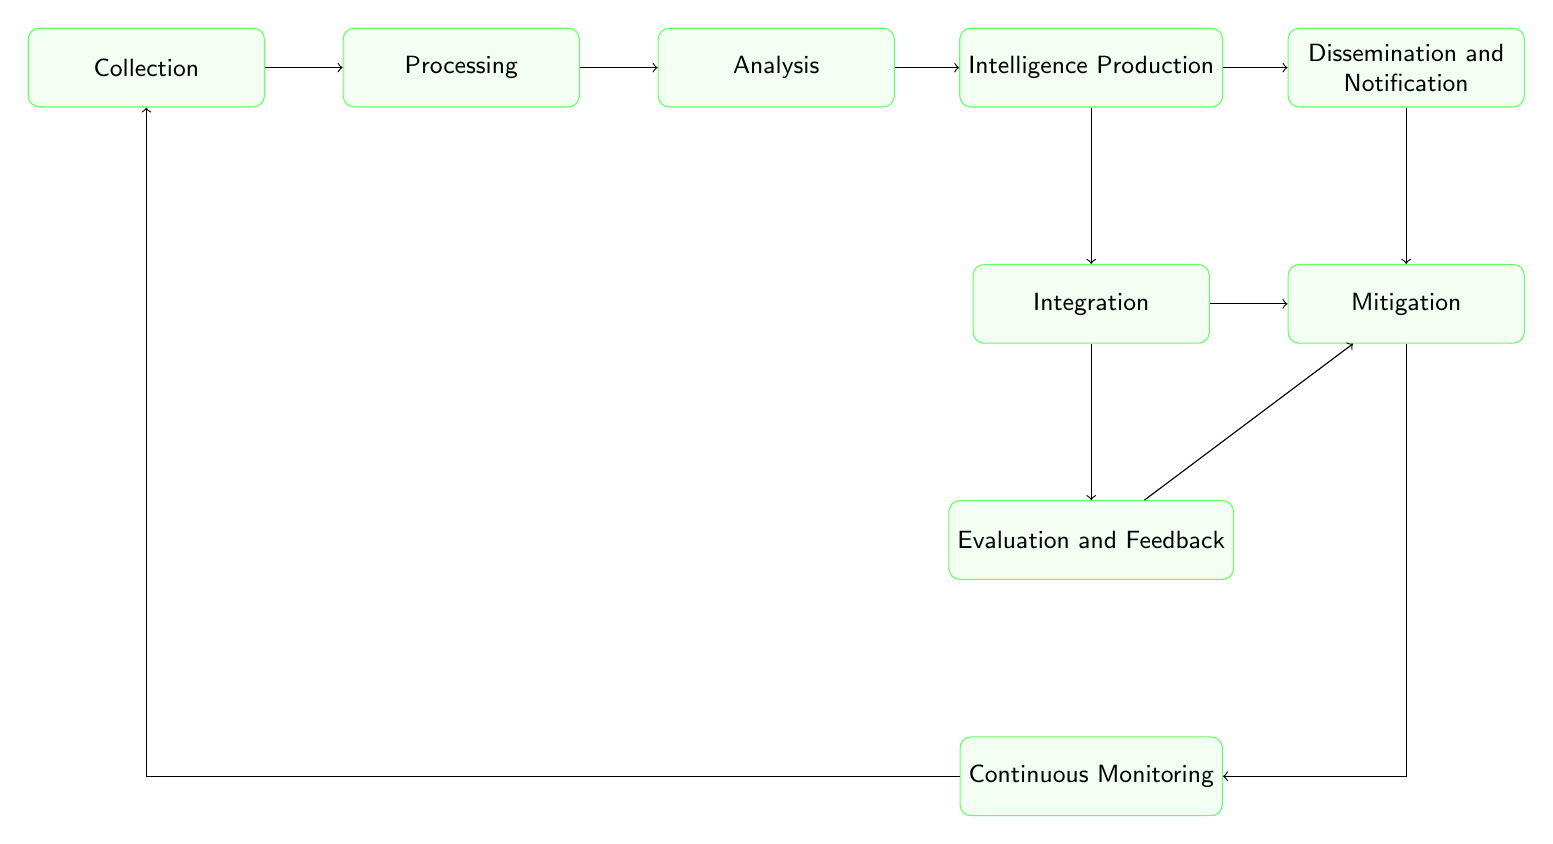
\begin{tikzpicture}[node distance=1.5cm, tblock/.style = {draw, trapezium, minimum height=10mm, 
                 trapezium left angle=75, trapezium right angle=105, align=center}, block/.style = {draw, rectangle, draw=green!60, fill=green!5, minimum height=10mm, minimum width=28mm,align=center}]

\tikzset{every node}=[font=\small\sffamily]
% Nodes
\node (collection) [block, rounded corners, minimum width=3cm, minimum height=1cm, text centered] {Collection};
\node (processing) [block, rounded corners, minimum width=3cm, minimum height=1cm, text centered, right of=collection, xshift=2.5cm] {Processing};
\node (analysis) [block, rounded corners, minimum width=3cm, minimum height=1cm, text centered, right of=processing, xshift=2.5cm] {Analysis};
\node (production) [block, rounded corners, minimum width=3cm, minimum height=1cm, text centered, right of=analysis, xshift=2.5cm] {Intelligence Production};
\node (dissemination) [block, rounded corners, minimum width=3cm, minimum height=1cm, text centered, right of=production, xshift=2.5cm] {Dissemination and\\ Notification};
\node (integration) [block, rounded corners, minimum width=3cm, minimum height=1cm, text centered, below of=production, yshift=-1.5cm] {Integration};
\node (evaluation) [block, rounded corners, minimum width=3cm, minimum height=1cm, text centered, below of=integration, yshift=-1.5cm] {Evaluation and Feedback};
\node (mitigation) [block, rounded corners, minimum width=3cm, minimum height=1cm, text centered, below of=dissemination, yshift=-1.5cm] {Mitigation};
\node (monitoring) [block, rounded corners, minimum width=3cm, minimum height=1cm, text centered, below of=evaluation, yshift=-1.5cm] {Continuous Monitoring};

% Arrows
\draw [->] (collection) -- (processing);
\draw [->] (processing) -- (analysis);
\draw [->] (analysis) -- (production);
\draw [->] (production) -- (dissemination);
\draw [->] (production) -- (integration);
\draw [->] (dissemination) -- (mitigation);
\draw [->] (integration) -- (evaluation);
\draw [->] (evaluation) -- (mitigation);
\draw [->] (mitigation) |- (monitoring);
\draw [->] (monitoring) -| (collection);
\draw [->] (integration) -- (mitigation);
\end{tikzpicture}
\end{adjustbox}
\end{frame}

% LINKS
\begin{frame}
\frametitle{Links}
    \begin{itemize}
        \item AIL project \url{https://github.com/ail-project} ({\bf all components including feeders and crawler infrastructure})
        \item AIL framework \url{https://github.com/ail-project/ail-framework} ({\bf analysis framework})
        \item Training materials and slide deck \url{https://github.com/ail-project/ail-training}
    \end{itemize}
    \begin{figure}
        
\includegraphics[scale=0.10, angle=0]{images/ail-project.png}
    \end{figure}
\end{frame}

\end{document}

